\documentclass[pdf,serif]{beamer}

\usepackage[orientation=poster,size=custom,width=76.2,height=101.6,scale=1.6,debug]{beamerposter}

\mode<presentation>{
\usetheme{Morristown}
}

\usepackage[utf8]{inputenc}
\usepackage[urw-garamond]{mathdesign}
\usepackage[T1]{fontenc}
\usepackage{ebgaramond}
\usepackage{booktabs}
\usepackage{fancyref}
\usepackage{tabularx}
\usepackage{graphicx}
\usepackage{siunitx}
\sisetup{separate-uncertainty=true}
\usepackage{listings}
\usepackage{hyperref} % covered with beamer?
\hypersetup{
colorlinks=true,
urlcolor=blue
}
\usepackage[export]{adjustbox}
\usepackage{svg}
\usepackage{amsmath,amsthm,amssymb}
%\boldmath
% Uncomment next line to restore figure numbers if you like that sort of thing
\setbeamertemplate{caption}[numbered]

% if using ieee style citations
%\usepackage{cite}
% or uncomment next line for biology style references
\usepackage[round,authoryear]{natbib}

\title{Is momentum conserved?}
\author{Your Name and D Evangelista}
\institute{Morristown-Beard School}
\date{\today}

\begin{document}
\begin{frame}{}
\begin{columns}[T,totalwidth=\textwidth]
\begin{column}{14.33in}
\begin{minipage}[t][\textheight]{\linewidth}
\begin{abstract}
Momentum is the product of mass times velocity ($\vec{p}=m\vec{v}$). It is potentially useful for understanding the mechanics of collisions. We examined if momentum is conserved during inelastic collisions using an instrumented, one-dimensional test track. \textbf{We found... You will write one sentence to finish off the ABSTRACT summarizing what you found.}
\end{abstract}
\vfill
\begin{block}{Conservation of momentum could be a useful principle.}
\begin{itemize}
\item Application to collisions in which two bodies collide and stick (inelastic collisions) or bounce off one another (elastic collisions). 
\item If momentum is conserved during such collisions, it could be means to find the final velocities of each of the bodies. 
\item Define $p_0$ and $p_f$ as
\begin{align*}
p_0 &= m_1 v_1 + m_2 v_2\ \text{before collision} \\
p_f &= m_1 v_{1,f} + m_2 v_{2,f}\ \text{after collision}. 
\end{align*}
\item Test for momentum conservation by testing if $p_f=p_0$.
\end{itemize}
\end{block}
\vfill
\begin{block}{We measured momentum change during two-body collisions using an instrumented test track.}
\begin{figure}[h]
\begin{center}
%\includegraphics[width=\columnwidth]{IMG_6253.jpg}
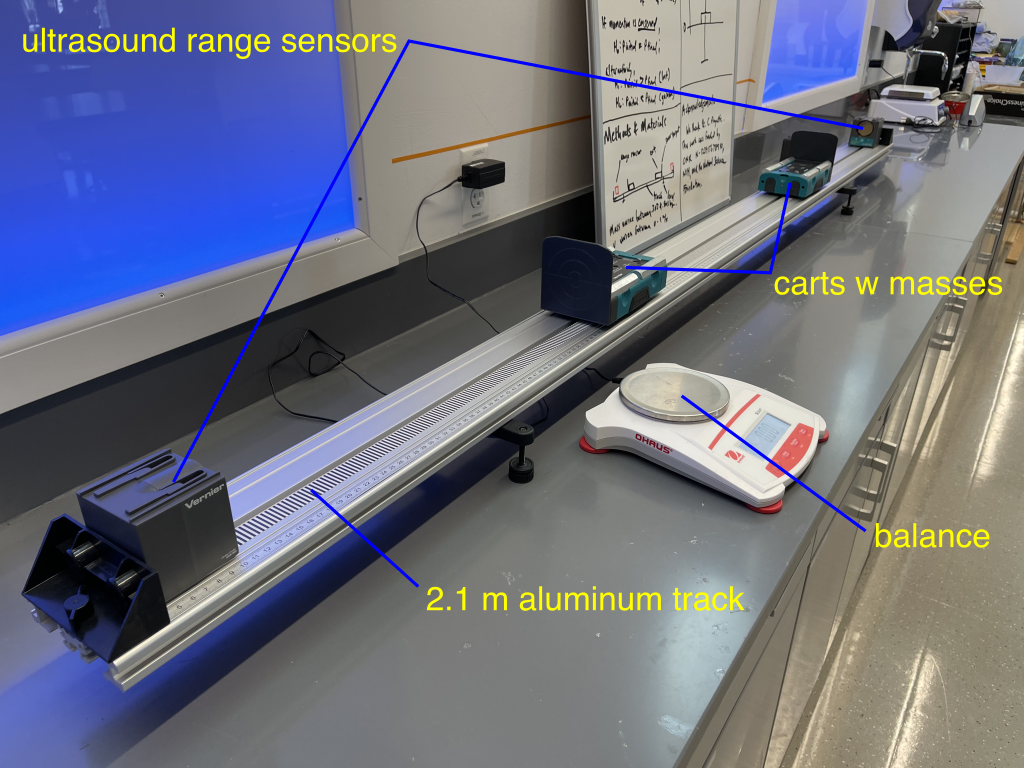
\includegraphics[width=0.8\columnwidth]{fig1.png}
\end{center}
\caption{Instrumented momentum test track used for experiments. Total length \SI{2.1}{\meter}. We tested $n=72$ collisions using masses between \SIrange{0.3}{0.8}{\kilo\gram} and speeds between \SIrange{0}{1.5}{\meter\per\second}. Position sensing with ultrasound range sensors; data logging via Bluetooth connection.}
\label{fig:methods1}
\end{figure}
\end{block}
\vfill
\end{minipage}
\end{column}

\begin{column}{14.33in}
\begin{minipage}[t][\textheight]{\linewidth}
\begin{block}{Inelastic collisions show $\Delta p\sim 0$.}
\begin{figure}
\begin{center}
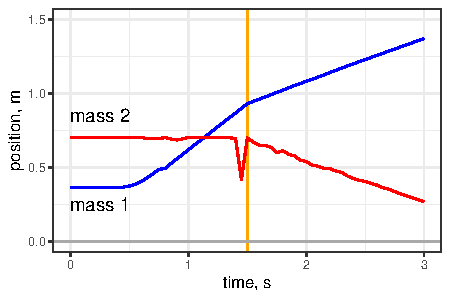
\includegraphics[width=0.8\columnwidth]{inelastic.pdf}
\end{center}
\caption{Position data for a typical inelastic collision with equal masses, $m_1=m_2=\SI{0.3}{\kilo\gram}$. Initially, $m_2$ is stationary and $m_1$ is moving at \SI{0.62}{\meter\per\second} based on the slopes. The masses collide at $t=\SI{1.5}{\second}$. After the collision, $m_1$ and $m_2$ are both moving with velocity $v_f=\SI{0.3}{\meter\per\second}$. }
\label{fig:results1}
\end{figure}
\begin{figure}
\begin{center}
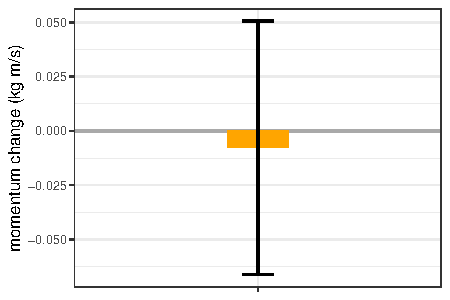
\includegraphics[width=0.8\columnwidth]{momentum-change.pdf}
\end{center}
\caption{Change in momentum ($\Delta p$) during all inelastic collisions. $\Delta p = \SI{-0.01\pm0.06}{\kilo\gram\meter\per\second}$ (mean $\pm$ s.d.). The mean $\Delta p$ is not significantly different from \SI{0}{\kilo\gram\meter\per\second} (one-sample $t$-test, $n=72$, d.f.=71, $p=0.2596$).}
\label{fig:results2}
\end{figure}
\end{block}
\vfill
\begin{block}{Place your bumper sticker here.}
\textbf{You will write a bulletized version of your findings here.  Were any of the hypotheses supported? Were any refuted with the observed data? Based on your observations, is momentum conserved, or is it gained, or lost, during the collisions you have tested? What does it all mean, big picture?}
\end{block}
\vspace{1.25in}
\begin{block}{} %Acknowledgements}
We thank C.~Payette, J.~Bartholomew, B.~Turner, and S.~McCormick; A.~Hahn and S.~Kealy. Support from the Alumni Association at Morristown-Beard School; ONR, AFOSR, NIH, and NSF.
\end{block}
\vfill*
\end{minipage}
\end{column}
\end{columns}
\end{frame}
\end{document}